    %?%%%%%%%%%%%%%%%%%%%%%%%%%%%%% HIPOTEZY %%%%%%%%%%%%%%%%%%%%%%%%%%%%%%
    \subsection{Hipotezy}
    Głównym celem badania było sprawdzenie, czy kolor okularów wpływa na czas skupienia (fiksacji) na żółtej torbie.
    W ramach tego celu sformułowano następujące hipotezy:
    \begin{itemize}
        \item $H_0$: Średnie czasy skupienia na żółtej torbie są równe dla wszystkich grup kolorów okularów.
        \item $H_1$: Nie dla wszystkich grup kolorów okularów średnie czasy skupienia na żółtej torbie są równe.
    \end{itemize}
    
    Dodatkowo, w ramach badania, sprawdzono wpływ doświadczenia zawodowego na czas skupienia na żółtej torbie.
    W tym celu sformułowano następujące hipotezy:
    \begin{itemize}
        \item $H_0$: Nie ma różnicy w czasie skupienia na żółtej torbie pomiędzy grupami z doświadczeniem i bez doświadczenia.
        \item $H_1$: Grupa z doświadczaniem ma dłuższy czas skupienia na żółtej torbie niż grupa bez doświadczenia.
    \end{itemize}
    
    %?%%%%%%%%%%%%%%%%%%%%%%%%%%%%% Analiza deskryptywna %%%%%%%%%%%%%%%%%%%%%%%%%%%%%%
    \subsection{Analiza deskryptywna zmiennej}
    \begin{table}[H]
        \centering
        \caption{Opis deskryptywny zmiennej TFD dla obiektu żółta torba (yellow bag).}
        \begin{tabular}{|c|c|c|c|}%
            \hline
            \bfseries Miara & \bfseries Gogle przezroczyste & \bfseries Gogle czerwone & \bfseries Gogle żółte% specify table head
            \csvreader[head to column names]{./../res_tables/summaryTFD_yBag.csv}{}% use head of csv as column names
            {\\\hline\Miara & \num{\T} & \num{\R} & \num{\Y}}% specify your columns here
            \\\hline    
        \end{tabular}
        \label{tab:summaryTFD_yBag}
    \end{table}
    \begin{figure}[H]
        \centering
        \resizebox{0.7 \columnwidth}{!}{%
        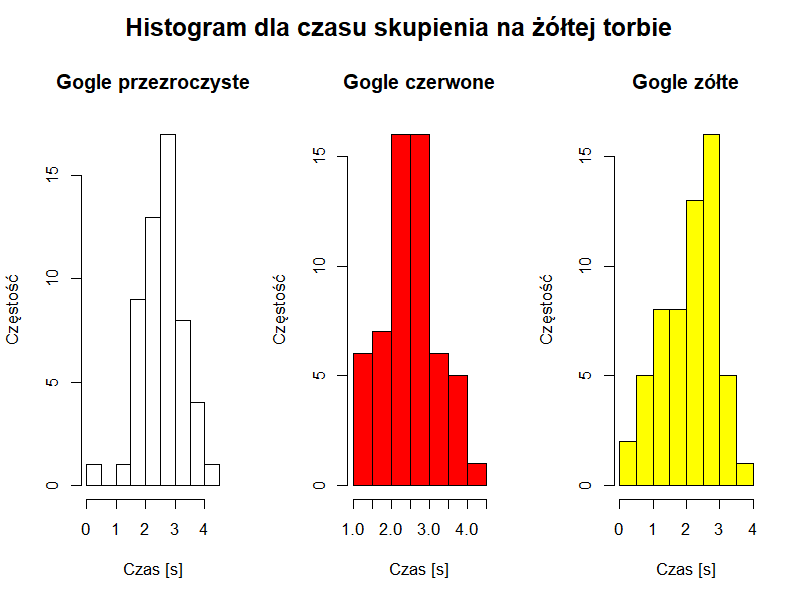
\includegraphics{./../res_plots/Histogram_dla_czasu_skupienia_na_żółtej_torbie.png}%
        }
        \label{fig:histTFD_yBag}
        \caption{Histogram dla zmiennej TFD dla obiektu żółta torba (yellow bag).}
    \end{figure}
    \begin{figure}[H]
        \centering
        \resizebox{0.7 \columnwidth}{!}{%
        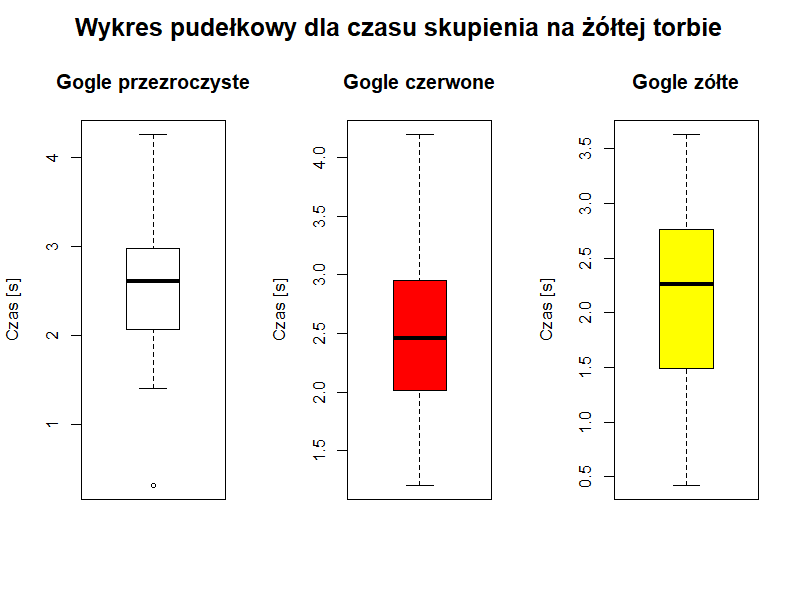
\includegraphics{./../res_plots/Wykres_pudełkowy_dla_czasu_skupienia_na_żółtej_torbie.png}%
        }
        \label{fig:boxTFD_yBag}
        \caption{Wykres pudełkowy dla zmiennej TFD dla obiektu żółta torba (yellow bag).}
    \end{figure}

    %?%%%%%%%%%%%%%%%%%%%%%%%%%%%%% Równoliczność grup %%%%%%%%%%%%%%%%%%%%%%%%%%%%%%
    \subsection{Równoliczność grup}
    Dla sprawdzenia równoliczności grup wykonano test $\chi^2$ z następującymi hipotezami:
    \begin{itemize}
        \item $H_0$: liczebności grup są równe.
        \item $H_1$: liczebności grup są różne.
    \end{itemize}
    Otrzymana wartość wynosi \textbf{$p=0.926$}, co oznacza, że na poziomie istotności $\alpha=0.05$
    nie ma podstaw do odrzucenia hipotezy zerowej. Na tej podstawie można stwierdzić, że \textbf{liczebności grup są równe}.
    
    %?%%%%%%%%%%%%%%%%%%%%%%%%%%%%% NORMALNOŚĆ %%%%%%%%%%%%%%%%%%%%%%%%%%%%%%

    \subsection{Normalność zmiennej w grupach}
    Do analizy normalności rozkładu zastosowane zostały histogramy oraz test Shapiro-Wilka. Oprócz analizy standardowych wartości
    zmiennej TFD-Y bag, przeprowadzono również analizy dla ich przekształceń: pierwiastek z X, pierwiastek kwadratowy z X oraz logarytm z X.

    \begin{table}[H]
        \centering
        \caption{Wyniki testu Shapiro-Wilka dla czasu skupienia na żółtej torbie (bez przekształceń).}
        \begin{tabular}{|c|c|c|}%
            \hline
            \bfseries Kolor okularów & \bfseries Wartość p & \bfseries Czy rozkład normalny% specify table head
            \csvreader[head to column names]{./../res_tables/yBag_shapiro_default.csv}{}% use head of csv as column names
            {\\\hline\kolorGogli & \num{\shapiroP} & \czyNormalny}% specify your columns here
            \\\hline    
        \end{tabular}
        \label{tab:shapiroYBagDefault}
    \end{table}
    \begin{figure}[H]
        \centering
        \resizebox{0.7 \columnwidth}{!}{%
        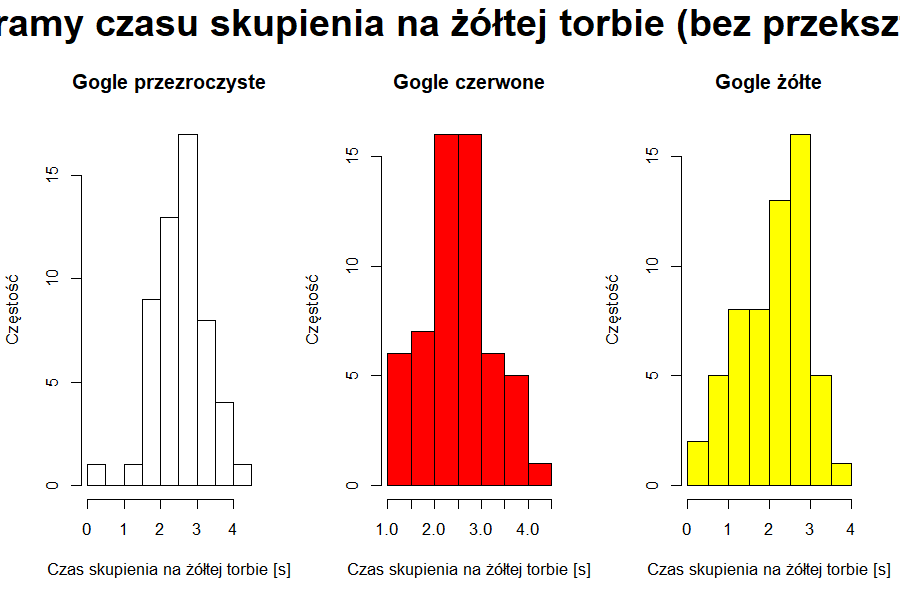
\includegraphics{./../res_plots/historgram_dla_TFD_yBag_default.png}%
        }
        \caption{Histogram dla czasu skupienia na żółtej torbie (bez przekształceń).}
        \label{fig:histYBagDefault}
    \end{figure}

    \begin{table}[H]
        \centering
        \caption{Wyniki testu Shapiro-Wilka dla czasu skupienia na żółtej torbie (pierwiastek z X).}
        \begin{tabular}{|c|c|c|}%
            \hline
            \bfseries Kolor okularów & \bfseries Wartość p & \bfseries Czy rozkład normalny% specify table head
            \csvreader[head to column names]{./../res_tables/yBag_shapiro_x^0.5.csv}{}% use head of csv as column names
            {\\\hline\kolorGogli & \num{\shapiroP} & \czyNormalny}% specify your columns here
            \\\hline    
        \end{tabular}
        \label{tab:shapiroYBagPow0.5}
    \end{table}
    \begin{figure}[H]
        \centering
        \resizebox{0.7 \columnwidth}{!}{%
        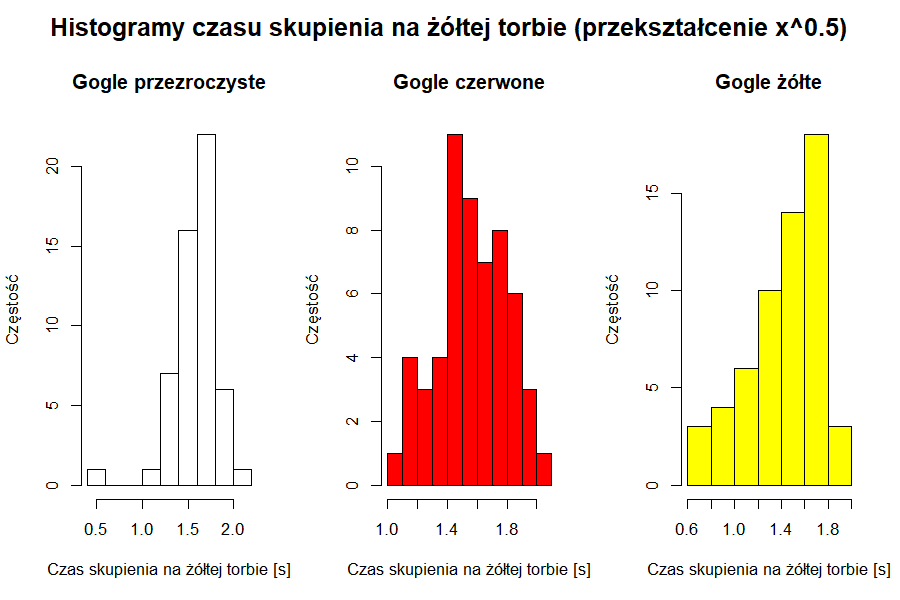
\includegraphics{./../res_plots/historgram_dla_TFD_yBag_x^0.5.png}%
        }
        \caption{Histogram dla czasu skupienia na żółtej torbie (pierwiastek z X).}
        \label{fig:histYBagPow0.5}
    \end{figure}

    \begin{table}[H]
        \centering
        \caption{Wyniki testu Shapiro-Wilka dla czasu skupienia na żółtej torbie (pierwiastek kwadratowy z X).}
        \begin{tabular}{|c|c|c|}%
            \hline
            \bfseries Kolor okularów & \bfseries Wartość p & \bfseries Czy rozkład normalny% specify table head
            \csvreader[head to column names]{./../res_tables/yBag_shapiro_x^0.25.csv}{}% use head of csv as column names
            {\\\hline\kolorGogli & \num{\shapiroP} & \czyNormalny}% specify your columns here
            \\\hline    
        \end{tabular}
        \label{tab:shapiroYBagPow0.25}
    \end{table}
    \begin{figure}[H]
        \centering
        \resizebox{0.7 \columnwidth}{!}{%
        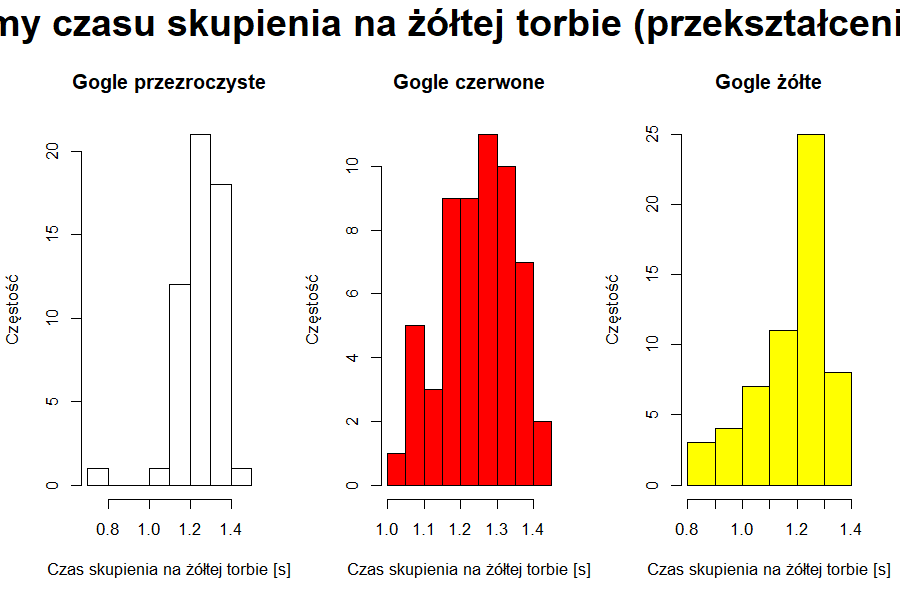
\includegraphics{./../res_plots/historgram_dla_TFD_yBag_x^0.25.png}%
        }
        \caption{Histogram dla czasu skupienia na żółtej torbie (pierwiastek kwadratowy z X).}
        \label{fig:histYBagPow0.25}
    \end{figure}

    \begin{table}[H]
        \centering
        \caption{Wyniki testu Shapiro-Wilka dla czasu skupienia na żółtej torbie (logarytm z X).}
        \begin{tabular}{|c|c|c|}%
            \hline
            \bfseries Kolor okularów & \bfseries Wartość p & \bfseries Czy rozkład normalny% specify table head
            \csvreader[head to column names]{./../res_tables/yBag_shapiro_log(x).csv}{}% use head of csv as column names
            {\\\hline\kolorGogli & \num{\shapiroP} & \czyNormalny}% specify your columns here
            \\\hline    
        \end{tabular}
        \label{tab:shapiroYBagLog}
    \end{table}
    \begin{figure}[H]
        \centering
        \resizebox{0.7 \columnwidth}{!}{%
        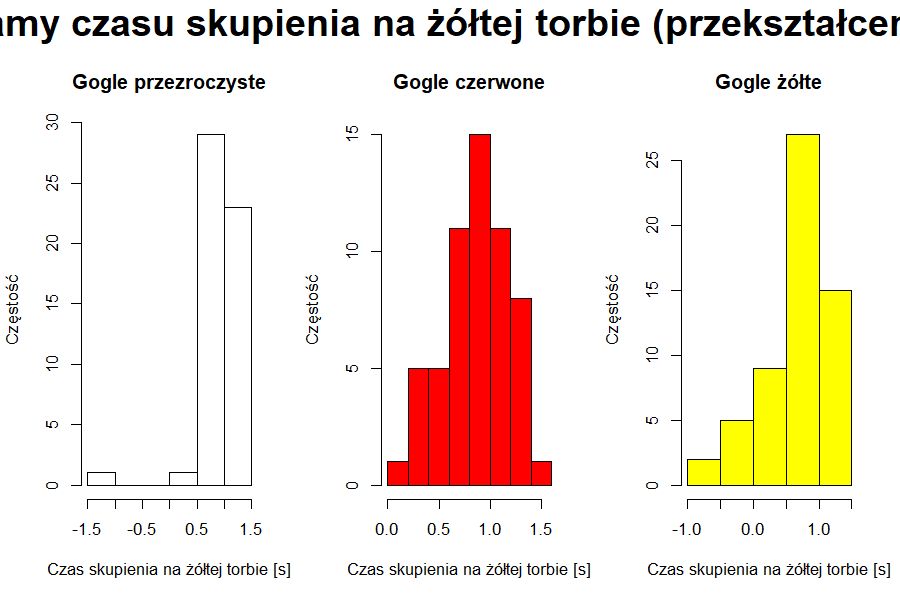
\includegraphics{./../res_plots/historgram_dla_TFD_yBag_log(x).png}%
        }
        \caption{Histogram dla czasu skupienia na żółtej torbie (logarytm z X).}
        \label{fig:histYBagLog}
    \end{figure}
   
    \begin{figure}[H]
        \centering
        \resizebox{0.7 \columnwidth}{!}{%
        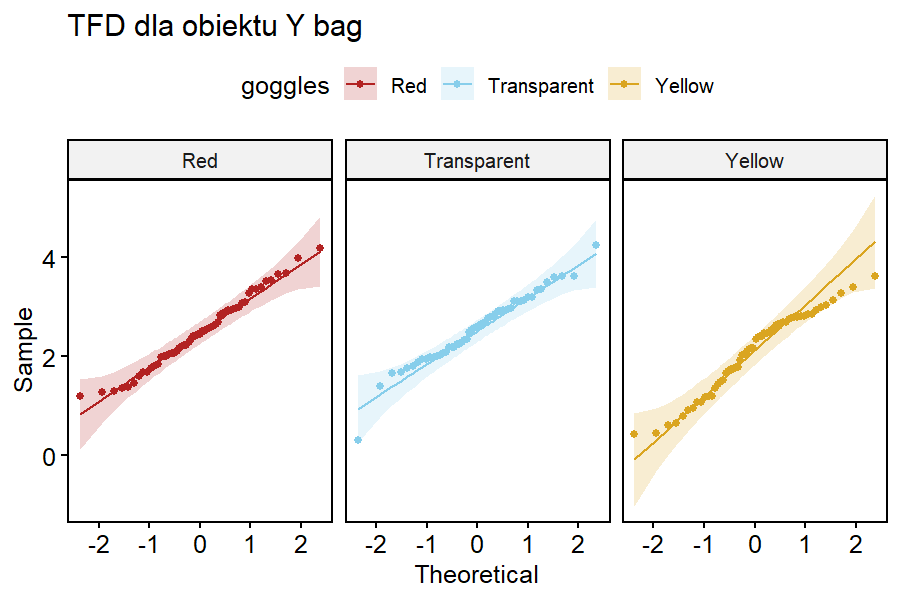
\includegraphics{./../res_plots/qqplot_dla_TFD_yBag.png}%
        }
        \caption{Wykres kwartyl-kwartyl dla czasu skupienia na żółtej torbie }
        \label{fig:qqplotYBag}
    \end{figure}
     
    Na podstawie otrzymanych histogramów [\ref{fig:histYBagDefault} - \ref{fig:histYBagLog}] i wyników testu Shapiro-Wilka 
    [\ref{tab:shapiroYBagDefault} - \ref{tab:shapiroYBagLog}] można stwierdzić, że \textbf{rozkłady są najbliższe normalności dla danych bez przekształceń}.
    Dla grupy czerwonej i przezroczystej wykonane testy wskazują na normalność rozkładu zmiennej TFD-Y bag.
    Dla grupy żółtej testy Shapiro-Wilka [\ref{tab:shapiroYBagDefault}] nie pozwala na przyjcie H0 świadczącej o normalności rozkładu,
    niemniej otrzymana wartość p jest bliska granicy istotności $\alpha=0.05$ oraz wykresy histogramu [\ref{fig:histYBagDefault}] i wykresy
    kwartyl-kwartyl [\ref{fig:qqplotYBag}] sugerują, że rozkład jest zbliżony do normalnego.
    Dlatego przyjęto, że \textbf{rozkład zmiennej TFD-Y bag jest normalny we wszystkich grupach}. 

    \subsection{Równość wariancji w grupach}
        Na podstawie wyników z sekcji \textit{''Normalność zmiennej w grupach''} stwierdzono, 
        normalność rozkładu zmiennej TFD-Y bag. Mając jednak na uwadze, że rozkład w grupie żółtej nie jest idealnie normalny, 
        przeprowadzono test Levene'a
        wycentrowanego na podstawie średniej, który jest bardziej odporny na odchylenia od normalności.

        Hipotezy:
        \begin{itemize}
            \item $H_0$: wariancje we wszystkich grupach są równe.
            \item $H_1$: co najmniej jedna grupa ma inną wariancję.
        \end{itemize}
        Otrzymana wartość wynosi $p=0.240$, co oznacza, że na poziomie istotności $\alpha=0.05$
        nie ma podstaw do odrzucenia hipotezy zerowej. Na tej podstawie można stwierdzić, że \textbf{wariancje są równe}.

    \subsection{Równość średnich w grupach}
        \subsubsection{Uzasadnienie wyboru testu}
        Na podstawie testów wykonanych w rozdziałach: \textit{''Równoliczność grup''}, 
        \textit{''Normalność zmiennej w grupach''} oraz \textit{''Równość wariancji w grupach''} ustalono, że rozkłady zmiennej TFD-Y bag
        w grupach są normalne, a liczebności i wariancje są równe. W związku z powyższym do porównania średnich
        w grupach zastosowano jednoczynnikową analizę wariancji testem \textbf{ANOVA}. Dodatkowo w analizę uzupełniono testem \textbf{post-hoc
        Tukeya} w celu określenia, które grupy różnią się od siebie.


        \subsubsection{Przeprowadzenie testu - wynik i wnioski}
        Hipotezy dla jednoczynnikowego testu ANOVA:
        \begin{itemize}
            \item $H_0$: średnie czasy skupienia na żółtej torbie są równe dla wszystkich grup kolorów okularów.
            \item $H_1$: przynajmniej jedna para średnich czasów skupienia na żółtej torbie jest istotnie różna.
        \end{itemize}

        Hipotezy dla testu Tukeya (dla każdej pary grup):
        \begin{itemize}
            \item $H_0$: średnie czasy skupienia na żółtej torbie są równe dla danej pary grup kolorów okularów.
            \item $H_1$: średnie czasy skupienia na żółtej torbie są różne dla danej pary grup kolorów okularów.
        \end{itemize}

        Dla przeprowadzonego testu ANOVA otrzymano wartość $p=0.002$, co oznacza, że na poziomie istotności $\alpha=0.05$
        można odrzucić hipotezę zerową. Na tej podstawie można stwierdzić, że \textbf{średnie czasy skupienia na żółtej torbie są różne dla przynajmniej jednej pary grup kolorów okularów}.

        Dla przeprowadzonego testu Tukeya otrzymano następujące wyniki:
        \begin{table}[H]
            \centering
            \caption{Wyniki testu post-hoc Tukeya}
             \begin{tabular}{|ll|cl}
            \cline{1-2}
            \multicolumn{2}{|c|}{\textbf{Kolor   okularów}}                                         & \textbf{}                               & \multicolumn{1}{c}{\textbf{}}          \\ \hline
            \multicolumn{1}{|c|}{\textbf{Grupa 1}} & \multicolumn{1}{c|}{\textbf{Grupa 2}} & \multicolumn{1}{c|}{\textbf{Wartość p}} & \multicolumn{1}{c|}{\textbf{Rezultat}} \\ \hline
            \multicolumn{1}{|l|}{czerwony}         & przezroczysty                         & \multicolumn{1}{c|}{0.868}              & \multicolumn{1}{l|}{H0 przyjęte}       \\ \hline
            \multicolumn{1}{|l|}{czerwony}         & żółty                                 & \multicolumn{1}{c|}{0.013}              & \multicolumn{1}{l|}{H0 odrzucone}      \\ \hline
            \multicolumn{1}{|l|}{przezroczysty}    & żółty                                 & \multicolumn{1}{c|}{0.003}              & \multicolumn{1}{l|}{H0 odrzucone}      \\ \hline
            \end{tabular}
            \label{tab:Tukeya}
        \end{table}

        Na podstawie tabeli [\ref{tab:Tukeya}] można stwierdzić, że średnie czasy skupienia na żółtej torbie są równe dla grupy czerwonej i przezroczystej,
        natomiast różnią się dla grupy czerwonej i żółtej oraz grupy przezroczystej i żółtej. Dodając do tego wyniki zawarte w tabeli 
        [\ref{tab:summaryTFD_yBag}] można założyć, że \textbf{grupa żółta ma najkrótszy czas skupienia na żółtej torbie}.

    \subsection{Wpływ doświadczenia zawodowego na zmienną TFD-Y bag}
    Dodatkowo, w ramach badania, sprawdzono wpływ doświadczenia na czas skupienia na żółtej torbie.
    W przeprowadzonym badaniu doświadczenie jest binarne, uczestnik może mieć doświadczenie lub nie.
    
    \begin{table}[H]
        \centering
        \caption{Opis deskryptywny czasu skupienia na żółtej torbie w grupach z doświadczeniem i bez doświadczenia.}
        \begin{tabular}{|c|c|c|}%
            \hline
            \bfseries Miara & \bfseries Z doświadczeniem & \bfseries Bez doświadczenia% specify table head
            \csvreader[head to column names]{./../res_tables/summaryExp_ybag.csv}{}% use head of csv as column names
            {\\\hline\Miara & \num{\ZExp} & \num{\BezExp}}% specify your columns here
            \\\hline    
        \end{tabular}
        \label{tab:summaryExp_ybag}
    \end{table}

    Dla każdej z grup w pierwszym kroku przeprowadzono test Shapiro-Wilka w celu sprawdzenia normalności rozkładu zmiennej TFD-Y bag.
    Przyjęte hipotezy:
    \begin{itemize}
        \item $H_0$: rozkład zmiennej TFD-Y bag jest normalny.
        \item $H_1$: rozkład zmiennej TFD-Y bag jest inny niż normalny.
    \end{itemize}
    Dla grupy z doświadczeniem otrzymano wartość $p=0.302$, z kolei dla grupy bez doświadczenia $p=0.910$. Dla obu grup nie ma podstaw do odrzucenia hipotezy zerowej.
    Na tej podstawie można stwierdzić, że \textbf{rozkład zmiennej TFD-Y bag jest normalny w obu grupach}.

    W związku ze ściśle normalnym rozkładem zmiennej w obu grupach do sprawdzenia jednorodności wariancji zastosowano test \textbf{Test F (Fishera)}.
    Przyjęte hipotezy:
    \begin{itemize}
        \item $H_0$: wariancje w grupach są równe.
        \item $H_1$: wariancje w grupach są różne.
    \end{itemize}
    Otrzymana wartość $p=0.868$ oznacza, że na poziomie istotności $\alpha=0.05$ nie ma podstaw do odrzucenia hipotezy zerowej.
    Na tej podstawie można stwierdzić, że \textbf{wariancje są równe w obu grupach}.

    Z racji normalności rozkładów zmiennej oraz równością wariancji do porównania średnich w grupach zastosowano test \textbf{t-Studenta}.
    Przyjęte hipotezy:
    \begin{itemize}
        \item $H_0$: średnie czasy skupienia na żółtej torbie są równe dla grupy z doświadczeniem i bez doświadczenia.
        \item $H_1$: średnie czasy skupienia na żółtej torbie są większe dla grupy z doświadczeniem niż dla grupy bez doświadczenia.
    \end{itemize}

    Otrzymana wartość $p=0.185$ oznacza, że na poziomie istotności $\alpha=0.05$ nie ma podstaw do odrzucenia hipotezy zerowej.
    Na tej podstawie można stwierdzić, że \textbf{nie ma różnicy w długości czasu skupienia na żółtej torbie pomiędzy grupą z doświadczeniem i bez doświadczenia}.